\chapter{Especificaciones del horno simulado}

\par En este capítulo se describen las especificaciones del horno a simular, condiciones de operación de diseño y características mecánicas; también se detalla la composición del combustible y características del aire ambiental utilizado para la combustión.

\section{Descripción del horno a simular}
\par El horno seleccionado para simular en este proyecto fue uno de tipo cabina con serpentín horizontal de tiro natural, de fuego directo simple y de dos pasos para el fluido, descrito en la Figura \ref{fig:diagrama-vista}.
\par Esta basado en el horno de una unidad de destilación al vacío de una refinería en operación. El residuo de vacío, por tratarse de un fluido proveniente de la unidad de destilación atmosférica puede considerarse que la vaporización dentro del serpentín de tubos es muy baja y no se toma en cuenta en los cálculos.
\par Utilizando las condiciones de operación de una hoja de datos del horno de residuo de vacío, se estableció la condición de operación del horno simulado como se muestra en la Tabla \ref{tbl:capacidad}.
\begin{table}[H]\begin{center}
\caption[Condición de operación de diseño del horno]{Condición de operación de diseño del horno simulado}
\label{tbl:capacidad}\begin{tabular}{c|c|c|c|c}
Capacidad de carga& $\Delta$T& Flujo Vol.   & Grav. Esp.& Flujo Másico\\
23 MW 	          & 52 °C    & 15,723.0 m3/d& 0.84      & 15,723.0 toneladas/d
\end{tabular}\end{center}\end{table}
\begin{figure}[H]
\begin{center}
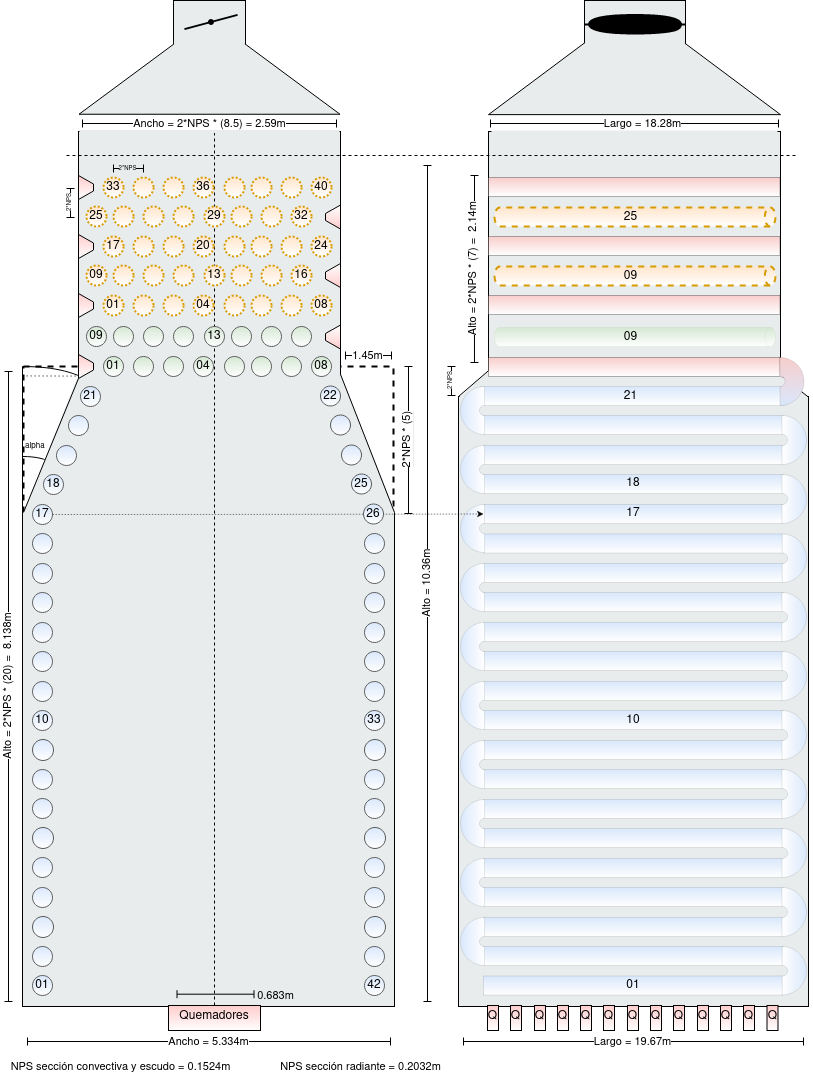
\includegraphics[scale=0.4]{images/diagrama-vista}
\caption[Cortes transversales del horno]{Cortes transversales del horno simulado.}
\label{fig:diagrama-vista}
\end{center}
\end{figure}

\subsection{Características mecánicas del horno seleccionado}
\par Lo primero a considerar en el diseño mecánico del horno fueron los tubos, se colocaron suficientes tubos para permitir la transferencia de calor equivalente a 70\% del calor requerido por el fluido de proceso en la sección de radiación.
\par El horno es de dos pasos, lo que significa que el fluido se divide en dos tuberías antes de ingresar, considerando la caída de presión para el diámetro nominal de los tubos. En la cámara de combustión, observada en la Figura \ref{fig:firebox}, se definió el ancho para cumplir con la relación alto/ancho establecida en el estándar API 560 \cite{bib:api560} y el resto de las medidas provienen de la separación y distribución de los tubos por sección sugeridas por el estándar.
\par En la Tabla \ref{tbl:firebox} se muestran las dimensiones resultantes de la cámara de combustión, son mostradas en pies y metros para su correspondiente uso en el cálculo de \ac{mbl}, resultando en la Ecuación \ref{eq:mbl} para el horno simulado.
\par Se puede observar a detalle cada una de las dimensiones de la configuración del horno en la Figura \ref{apx:img} ampliada en los anexos.
\begin{figure}[hbt] \begin{center}
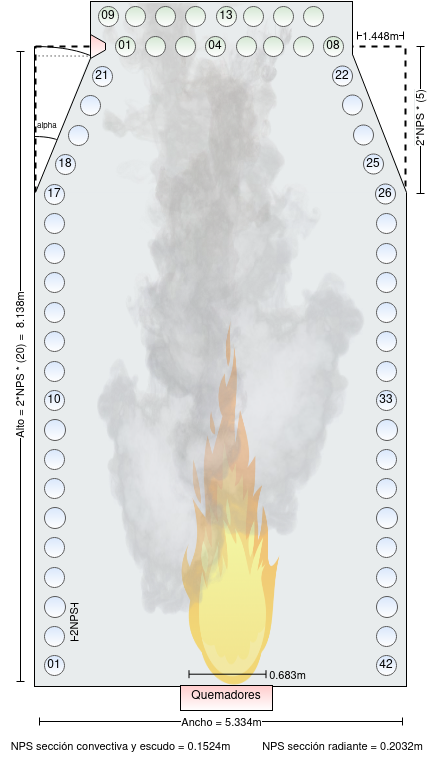
\includegraphics[scale=0.455]{images/firebox}
\caption[Diagrama de la cámara de combustión]{Diagrama de la cámara de combustión (sección radiante) del horno simulado.}
\label{fig:firebox} \end{center} \end{figure}
\begin{table}[H] \begin{center}
\caption[Dimensiones de la cámara de combustión]{Dimensiones de la cámara de combustión, mostrada en pies para su uso en la ecuación \ref{eq:pl} y la Tabla \ref{tbl:mbl}}
\label{tbl:firebox} \begin{tabular}{c|c|c}
Altura interna	&  8.354 m & 27.407 ft\\
Largo interno 	& 19.675 m & 64.552 ft\\
Ancho interno 	&  5.334 m & 17.500 ft\\
\end{tabular} \end{center} \end{table}
\begin{equation} \label{eq:mbl}
    MBL = 2/3 * (Alto*Largo*Ancho)^{1/3} = 20.829ft = 6.349m
\end{equation}
\par La descripción detallada de las característica de los tubos y aletas usadas se puede encontrar en la Tabla \ref{tbl:tubes} y una vista en perspectiva de la distribución de los tubos se puede apreciar en la Figura \ref{fig:diagrama-vista} al inicio de este capítulo.
\begin{table}[hbt]
\begin{center}
\caption[Distribución de tubos en el horno]{Distribución de tubos en el horno}
\label{tbl:tubes}
\begin{tabular}{l|c|c|c}
Sección 					& Radiante	& Escudo		& Convectiva \\
\hline
Material de tubos			& \multicolumn{3}{c}{-- A-312 TP321 --} \\

Soporte de tubos    		& Interno	& Externo		& Externo		\\
Arreglo	de tubos    		& Paralelo	& Escalonado	& Escalonado	\\
No. de pasos del fluido		& 2	        & 2	            & 2	            \\
No. de tubos total    		& 42		& 16			& 40			\\
No. de tubos por fila		& 2			& 8				& 8				\\
Grosor pared de tubos, cm	& 0.818		& 0.711			& 0.711			\\
Di. interno de tubos, cm	& 7.981		& 16.827		& 16.827		\\
Espaciado de tubos, cm  	& 40.640	& 				& 				\\
Espaciado transversal, cm  	&			& 30.480		& 30.480		\\
Espaciado longitudinal, cm 	&			& 30.480		& 30.480		\\
Largo de tubos efectivo, m	& 18.926    & 18.288		& 18.288		\\
\hline
Material de aletas			&			& 				& 11.5-13.5Cr	\\
Tipo de aletas				&			& 				& Solidas		\\	
Altura de aletas, cm		&			& 				& 2.438			\\
Grosor de aletas, cm		&			& 				& 0.152			\\
Densidad de aletas, aleta/m	&			& 				& 196.850		\\
\end{tabular} \end{center} \end{table}
\par La conductividad térmica de los tubos se calcula a traves de la ecuación:
\begin{equation}
k_w = (14.643 + 1.64e-2*T - 2e-6*T^2)*3.6 \quad [kJ/h.m^{\circ} C)]
\end{equation}
\par Se estableció que estas variables de diseño mecánico del horno no pueden ser modificadas por el usuario del simulador, a menos que se edite directamente el código.

\subsection{Condiciones de diseño para el combustible y el aire}
\par Como combustible se utilizó un gas de refinería por tratarse de un subproducto de las operaciones de refinación. La composición molar establecida por defecto, y usada para hacer la comprobación del algoritmo en el siguiente capítulo, se describe en la Tabla \ref{tbl:combustible}. Sin embargo, la posibilidad de cambiar la composición está abierta en la interfaz del simulador.
\par El aire ambiental establecido contiene humedad, definida a través de la humedad relativa y la temperatura; el cual en base seca solo considera nitrógeno y oxígeno, otros compuestos, como el argón, dióxido de carbono y otras trazas, son tomados dentro del contenido de nitrógeno por sus aportes del 1\% o menos a las ecuaciones de combustión.
\begin{table}[hbt]\begin{center}
\caption[Composición molar del gas de refinería]{Composición molar del gas de refinería para comprobación.}
\label{tbl:combustible}\begin{tabular}{l|r}
	Gas combustible					& (Moles \%) \\
	\hline
	Metano ($CH_4$)					& 56.47 \\
	Etano ($C_2H_6$)				& 15.15 \\
	Propano ($C_3H_8$)				& 6.22 \\
	n-Butano ($C_4H_{10}$)			& 1.76 \\
	i-Butano ($C_4H_{10}$)			& 0.75 \\
	Etileno ($C_2H_4$)				& 1.58 \\
	Propileno ($C_3H_6$)			& 2.77 \\
	Monóxido de carbono ($CO$)		& 0.66 \\
	Dióxido de carbono ($CO_2$)		& 2.54 \\
	Hidrógeno ($H_2$)				& 11.42 \\
	Nitrógeno ($N_2$)				& 0.68 \\
	Agua ($H_2O$)					& 0.00 \\
	Oxigeno ($O_2$)					& 0.00 \\
	Sulfuro de hidrógeno ($H_2S$)	& 0.00 \\
\end{tabular}\end{center}\end{table}
\par Como se describió en la sección de combustión del capítulo 2, la composición tomada para el aire seco es 20.95\% de oxígeno y 79.05\% de nitrógeno.
\begin{table}[hbt]\begin{center}
\caption[Características del aire]{Características del aire usado en la comprobación.}
\label{tbl:aire}\begin{tabular}{l|r}
	Exceso de aire, \%								& 20.000 \\
	Humedad relativa, \%							& 50.000 \\
	Temperatura del aire, °C						& 26.667 \\
\end{tabular}\end{center}\end{table}